\chapter{Resultados de los tests de inyecci\'on de se\~nal}
\label{app:si_results}


\paragraph{Se\`nales Gaussianas}

En las \Figrange{\ref{fig:si_results:siginj_gaus_SR}}{\ref{fig:si_results:siginj_gaus_SRB}}, se muestran los resultados del test de \ac{SI} con señales gaussianas para los diferentes anchos de \(\sigma_G/\mG = 0.02, \, 0.05\) y \(0.20\). Las pruebas se han realizado en cada una de las regiones de análisis: SR, SRL, SRC y SRB. Para todas las hipótesis de ancho de la distribuci\'on se supera el test ya que se observan comportamientos lineales, y la relación de \(\left|\sspur\right| / N_{\text{inj}} < 0.5\)


\begin{figure}[ht!]
    \centering
    \begin{subfigure}[h]{0.32\linewidth}
        \centering
        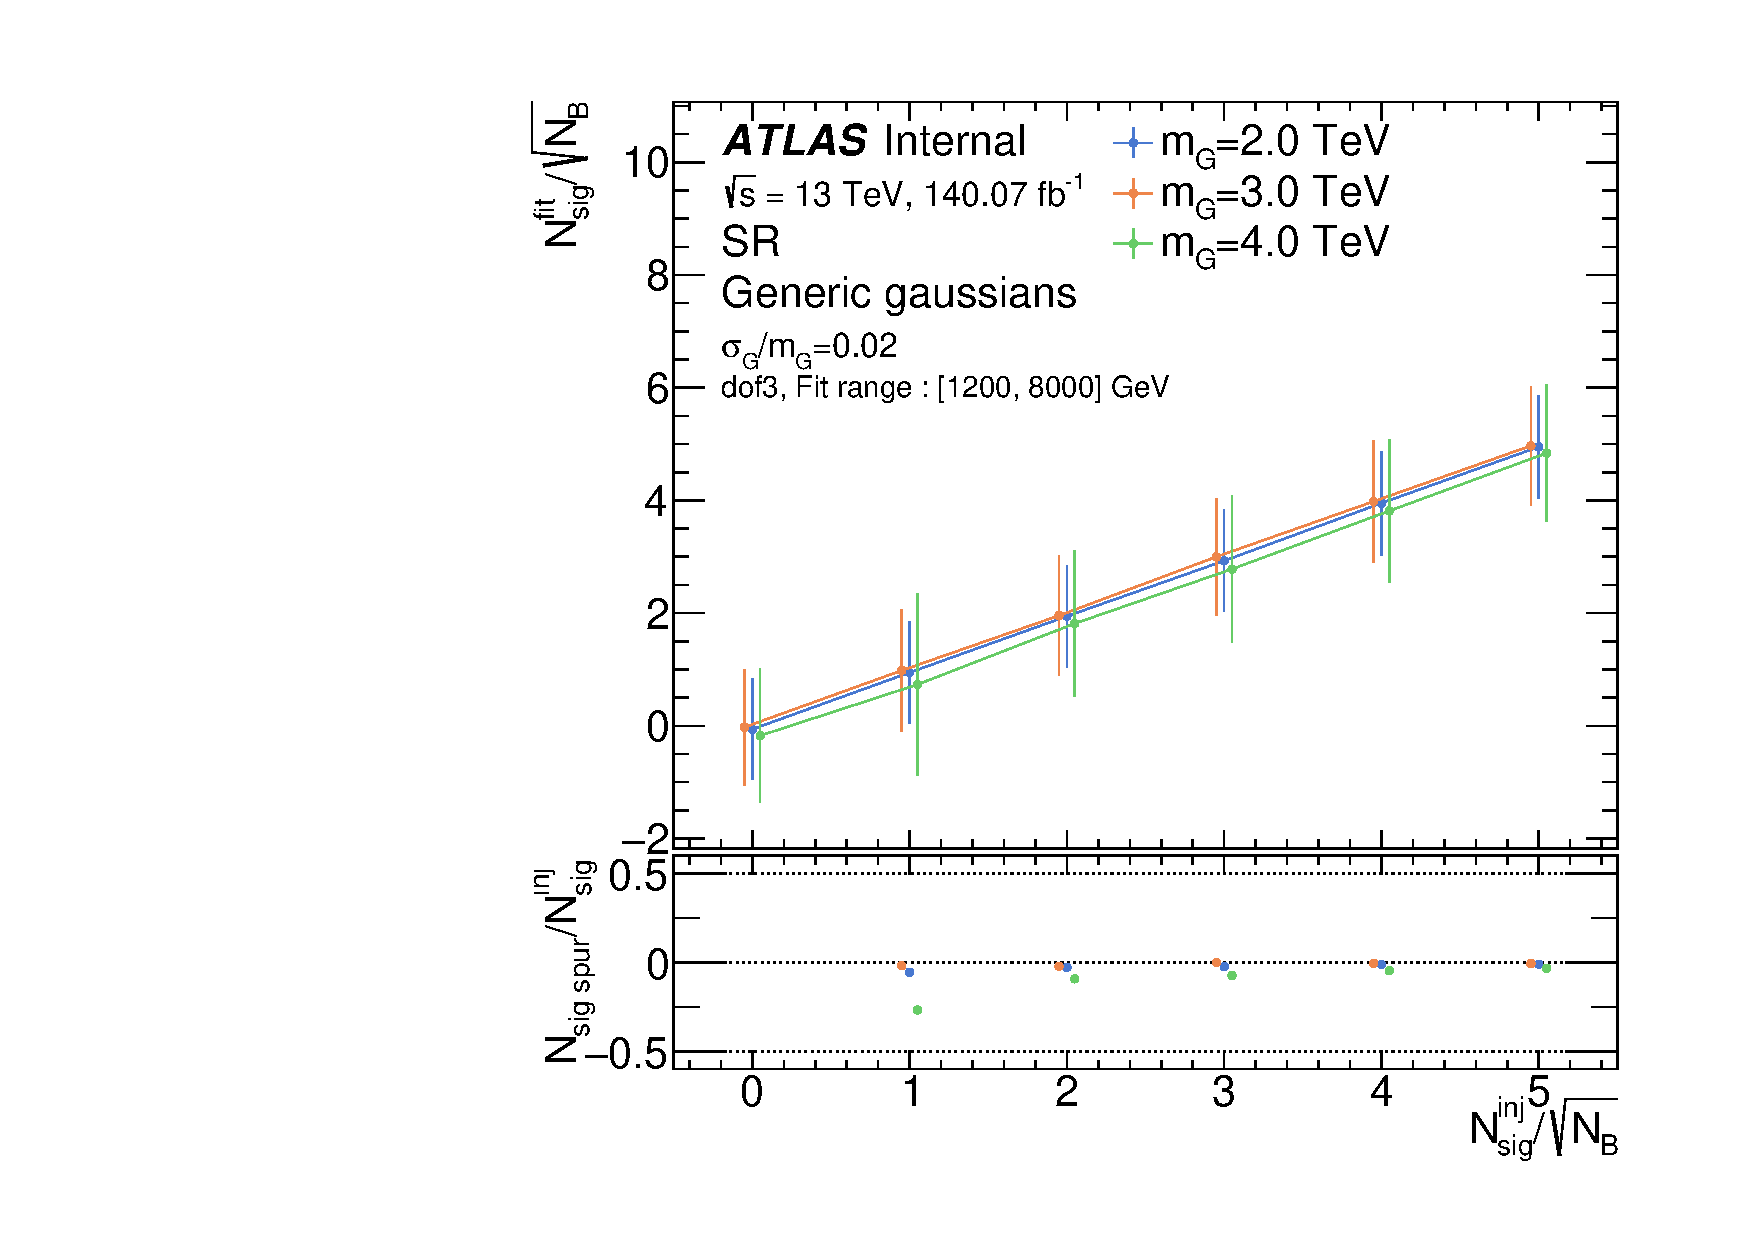
\includegraphics[width=\textwidth]{5_resonances/bkg/modeling/si/toys/SR/gaus/width0p02/dof3__range_1200_8000/plots/can__SigInj__photonjet_Pythia_jfakeisosmooth__gaus__SR__width0p02__dof3__range_1200_8000}
        \caption{\(\sigma_G/\mG = 0.02\).}
    \end{subfigure}
    \hfill
    \begin{subfigure}[h]{0.32\linewidth}
        \centering
        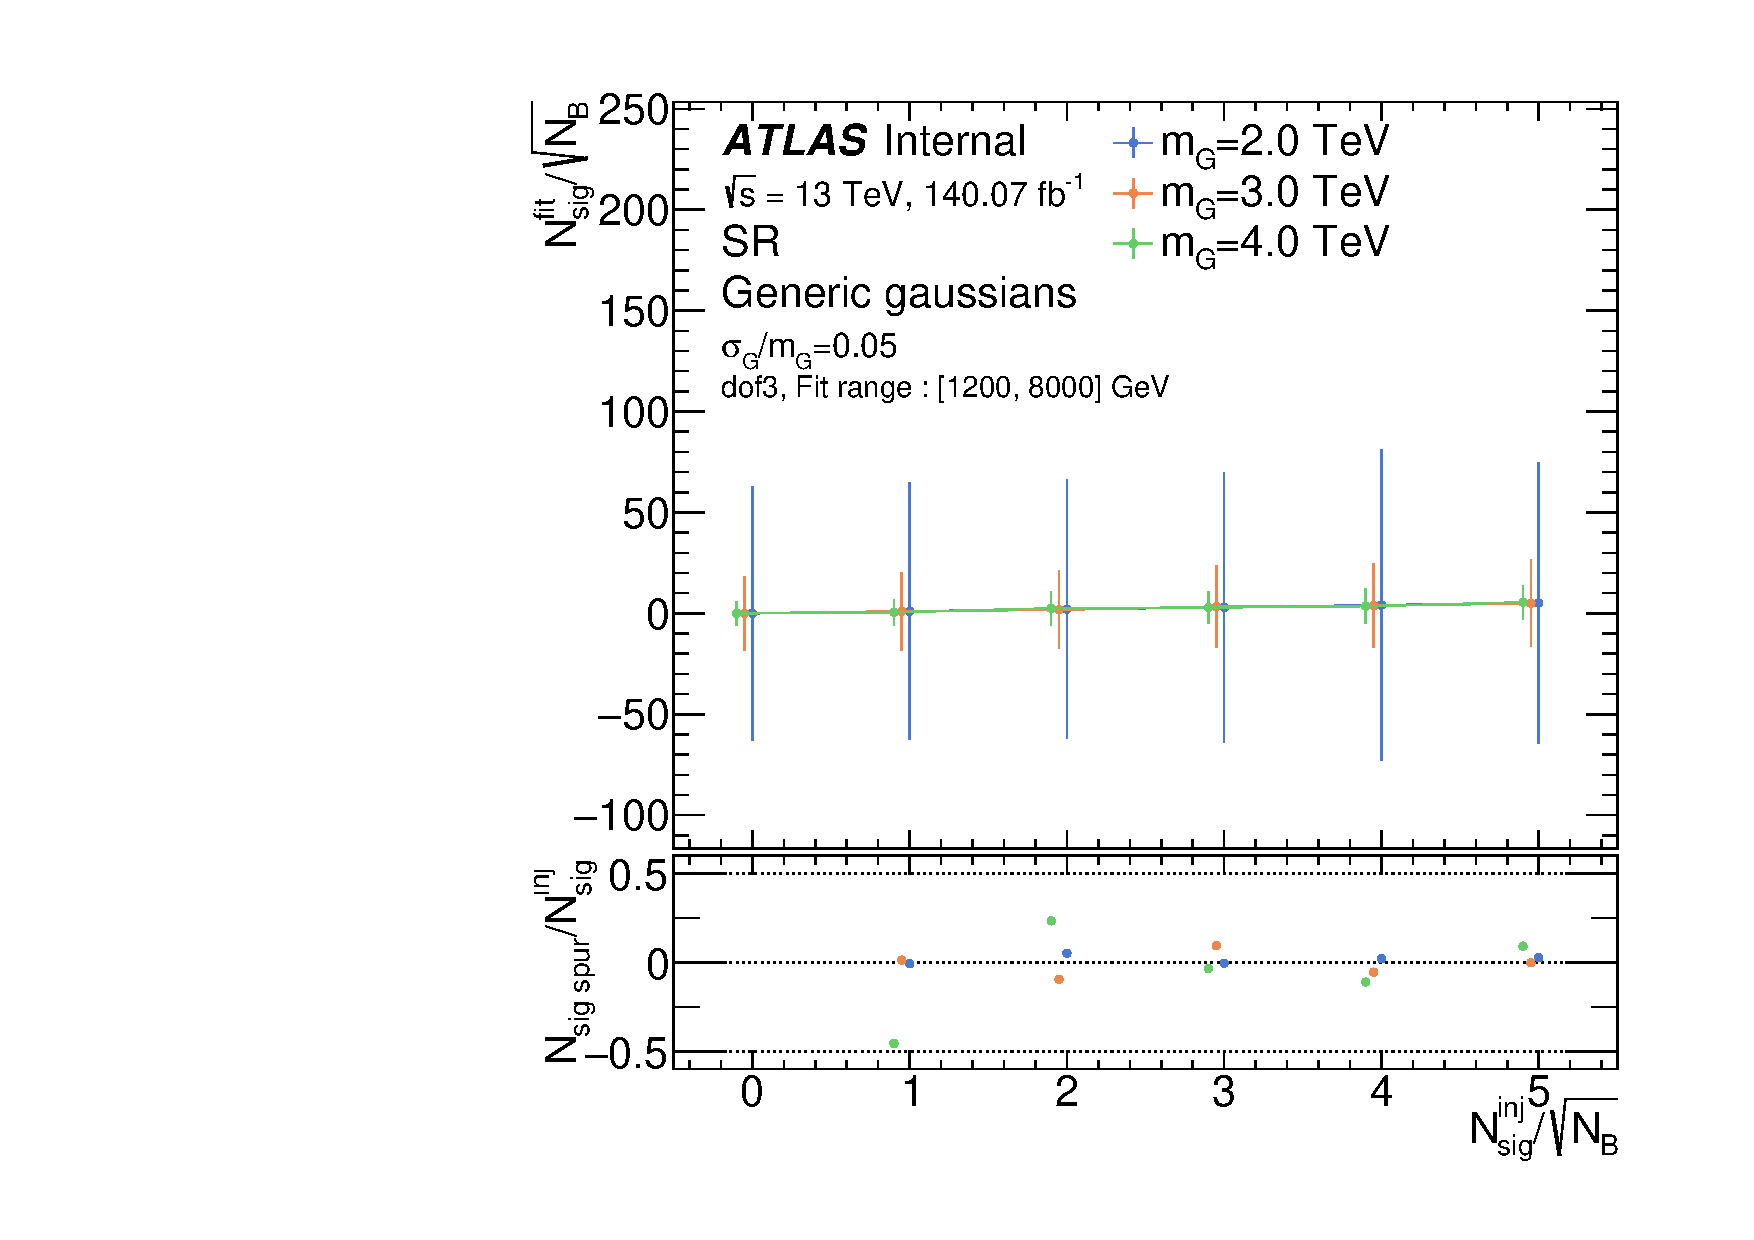
\includegraphics[width=\textwidth]{5_resonances/bkg/modeling/si/toys/SR/gaus/width0p05/dof3__range_1200_8000/plots/can__SigInj__photonjet_Pythia_jfakeisosmooth__gaus__SR__width0p05__dof3__range_1200_8000}
        \caption{\(\sigma_G/\mG = 0.05\).}
    \end{subfigure}
    \hfill
    \begin{subfigure}[h]{0.32\linewidth}
        \centering
        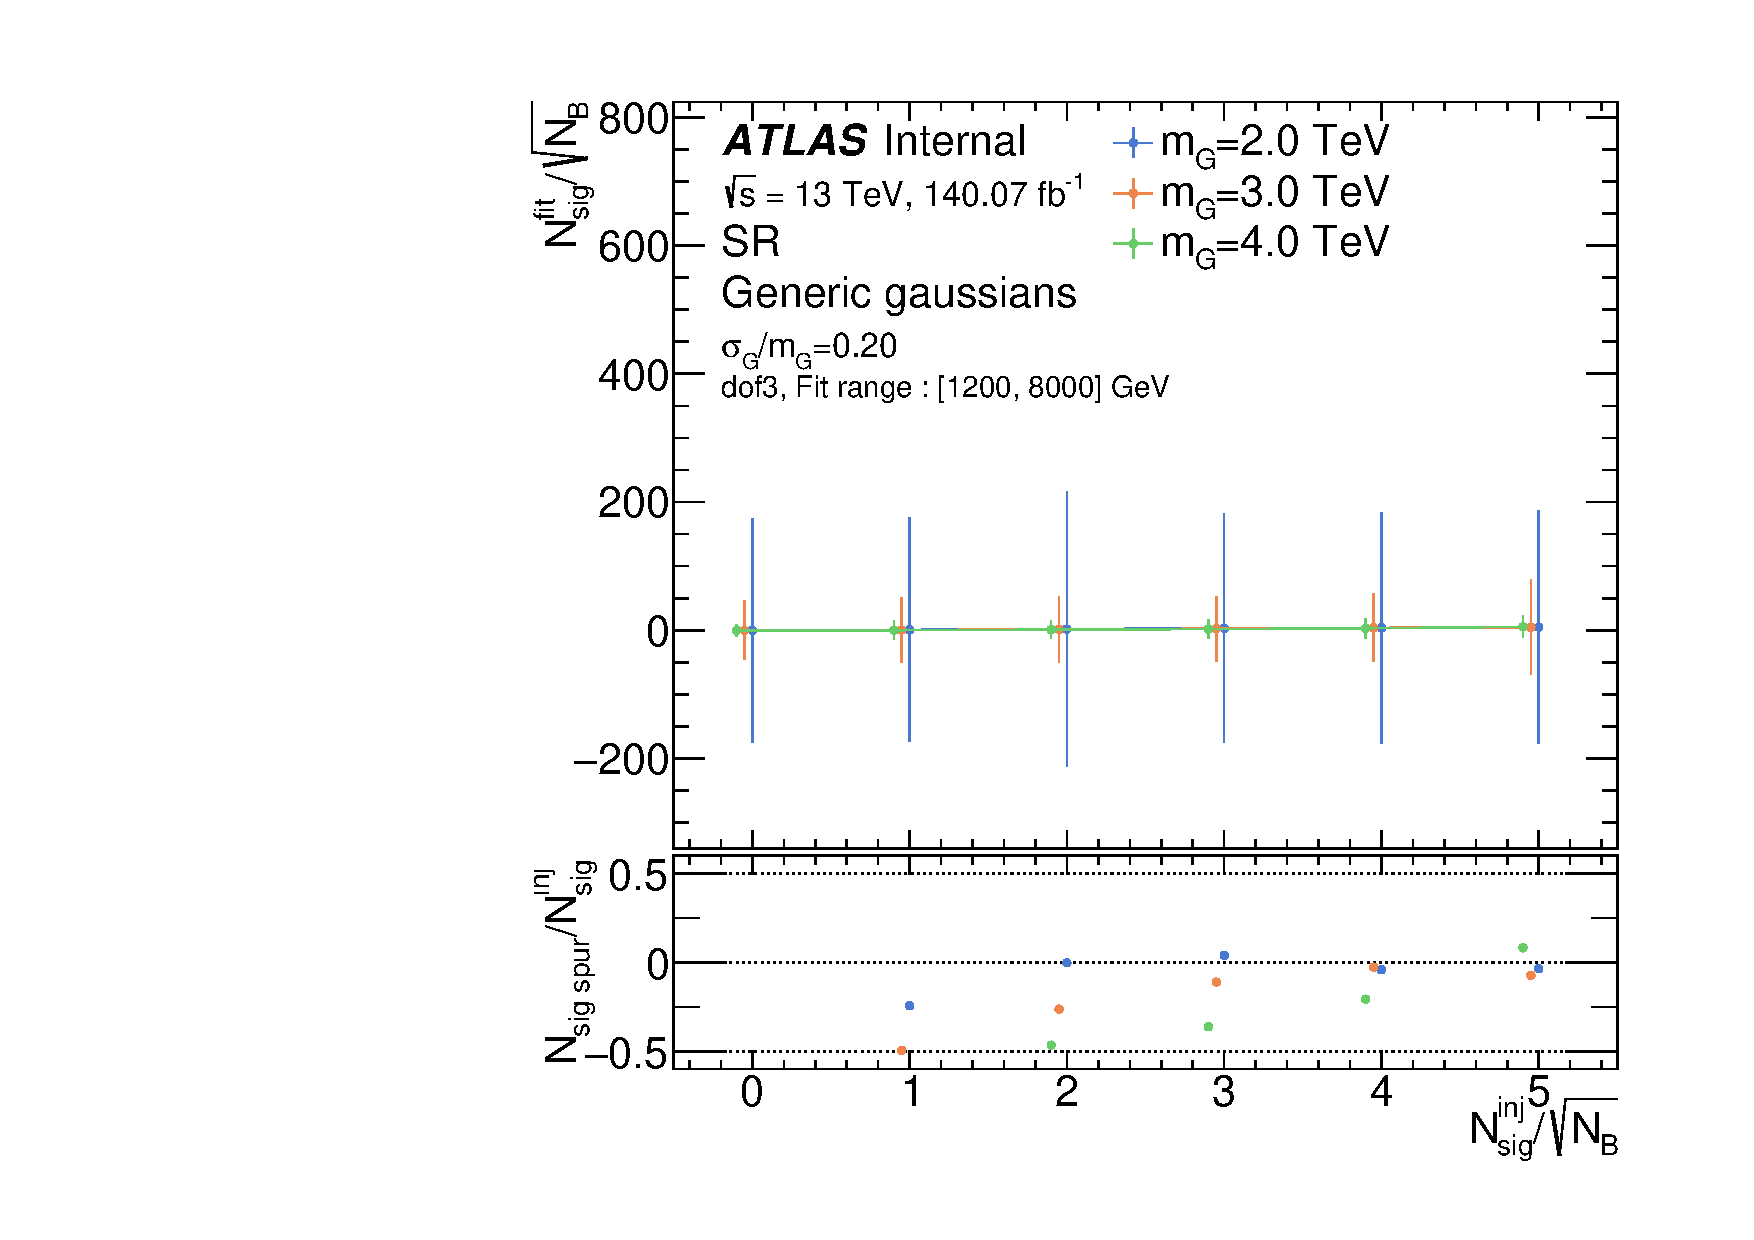
\includegraphics[width=\textwidth]{5_resonances/bkg/modeling/si/toys/SR/gaus/width0p20/dof3__range_1200_8000/plots/can__SigInj__photonjet_Pythia_jfakeisosmooth__gaus__SR__width0p20__dof3__range_1200_8000}
        \caption{\(\sigma_G/\mG = 0.20\).}
    \end{subfigure}
    \caption{Resultados de los tests de \ac{SI} usando se\~nales Gaussianasen la regi\'on inclusiva SR. El ajuste se realiza en el rango de \(1200-8000~\gev\) usando la funci\'on \textit{dof3}. Cada masa considerada se muestra con un color diferente. El eje \(x\) muestra la amplitud inyectada de se\~nal sobre el fondo, en unidades de \(\sqrt{N_B}\), mientras que el eje \(y\) representa la se\~nal extra\'idaen unidades de \(\sqrt{N_B}\).}
    \label{fig:si_results:siginj_gaus_SR}
\end{figure}

\begin{figure}[ht!]
    \centering
    \begin{subfigure}[h]{0.32\linewidth}
        \centering
        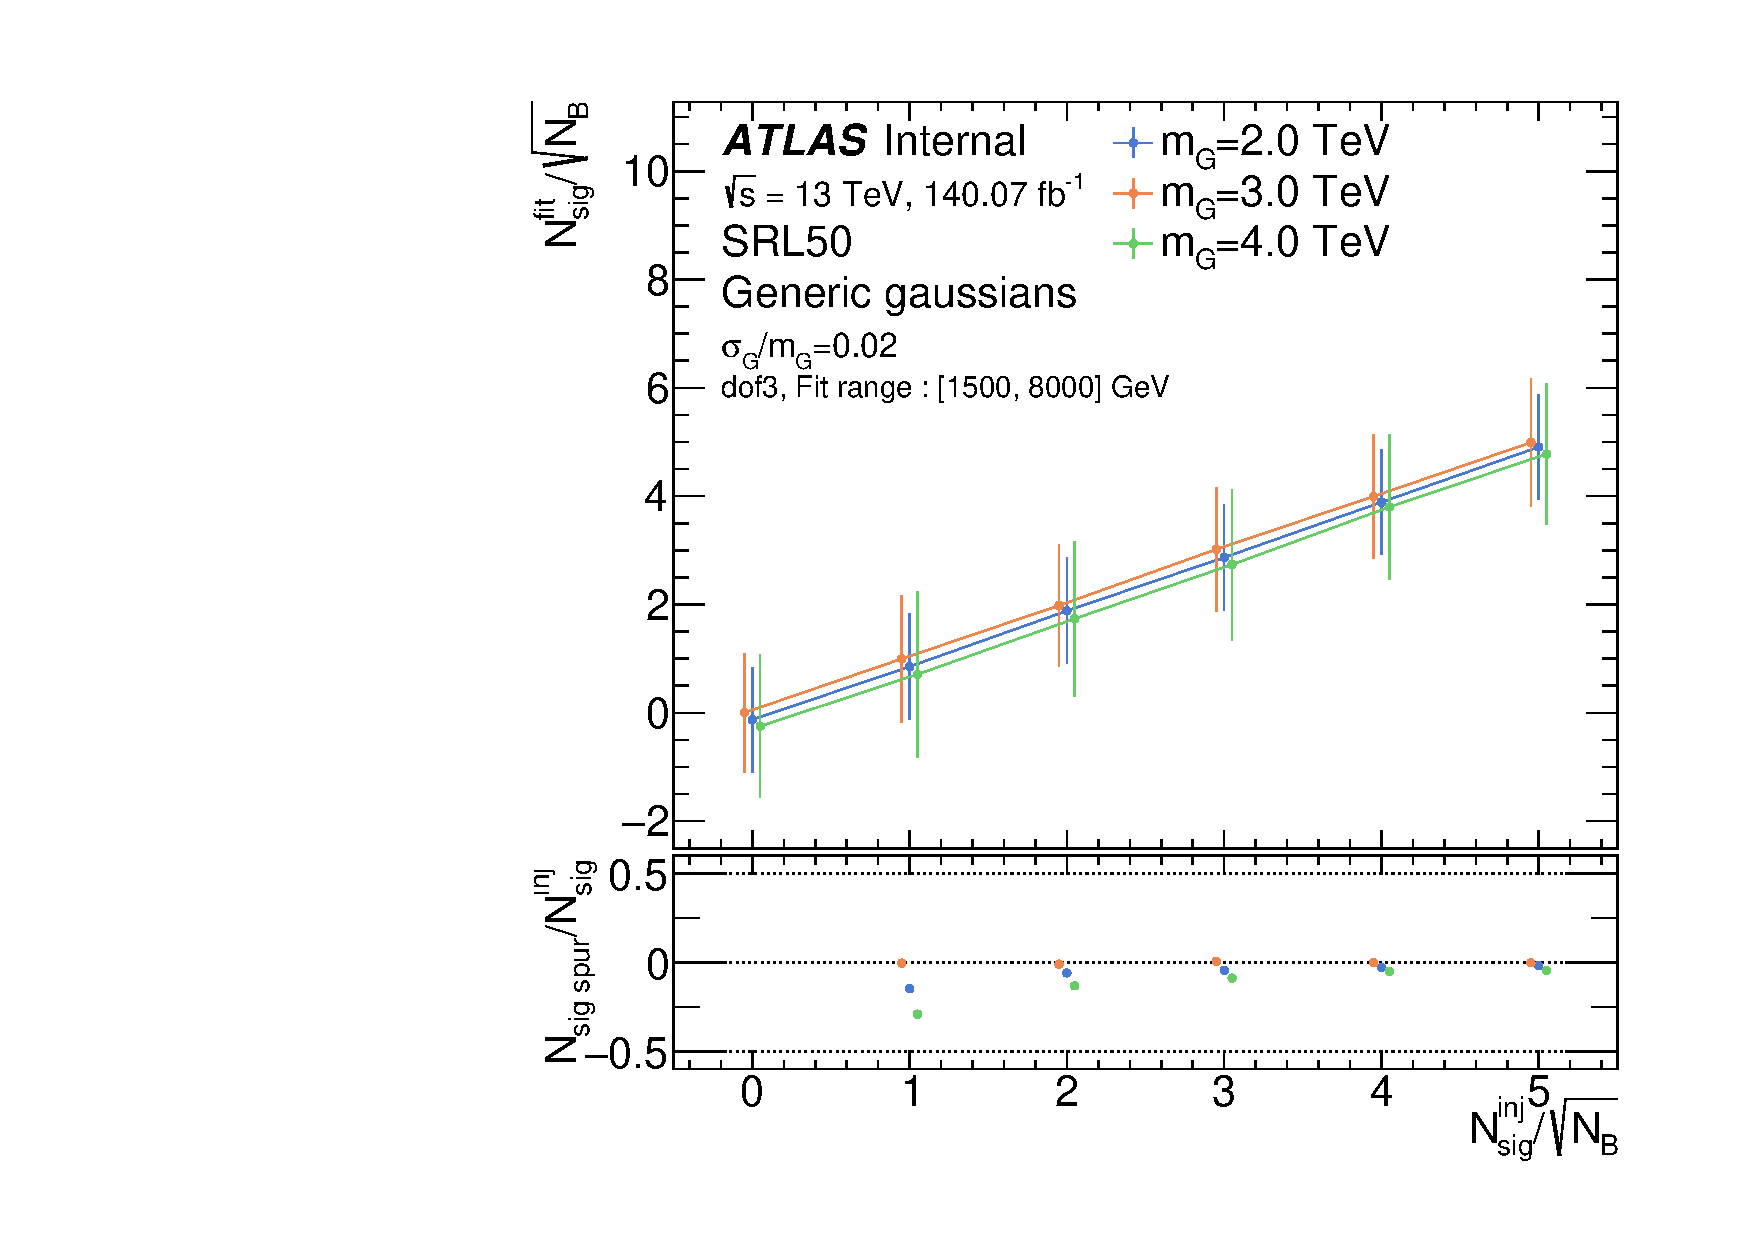
\includegraphics[width=\textwidth]{5_resonances/bkg/modeling/si/toys/SRL50/gaus/width0p02/dof3__range_1500_8000/plots/can__SigInj__photonjet_Pythia_jfakeisosmooth__gaus__SRL50__width0p02__dof3__range_1500_8000}
        \caption{\(\sigma_G/\mG = 0.02\).}
    \end{subfigure}
    \hfill
    \begin{subfigure}[h]{0.32\linewidth}
        \centering
        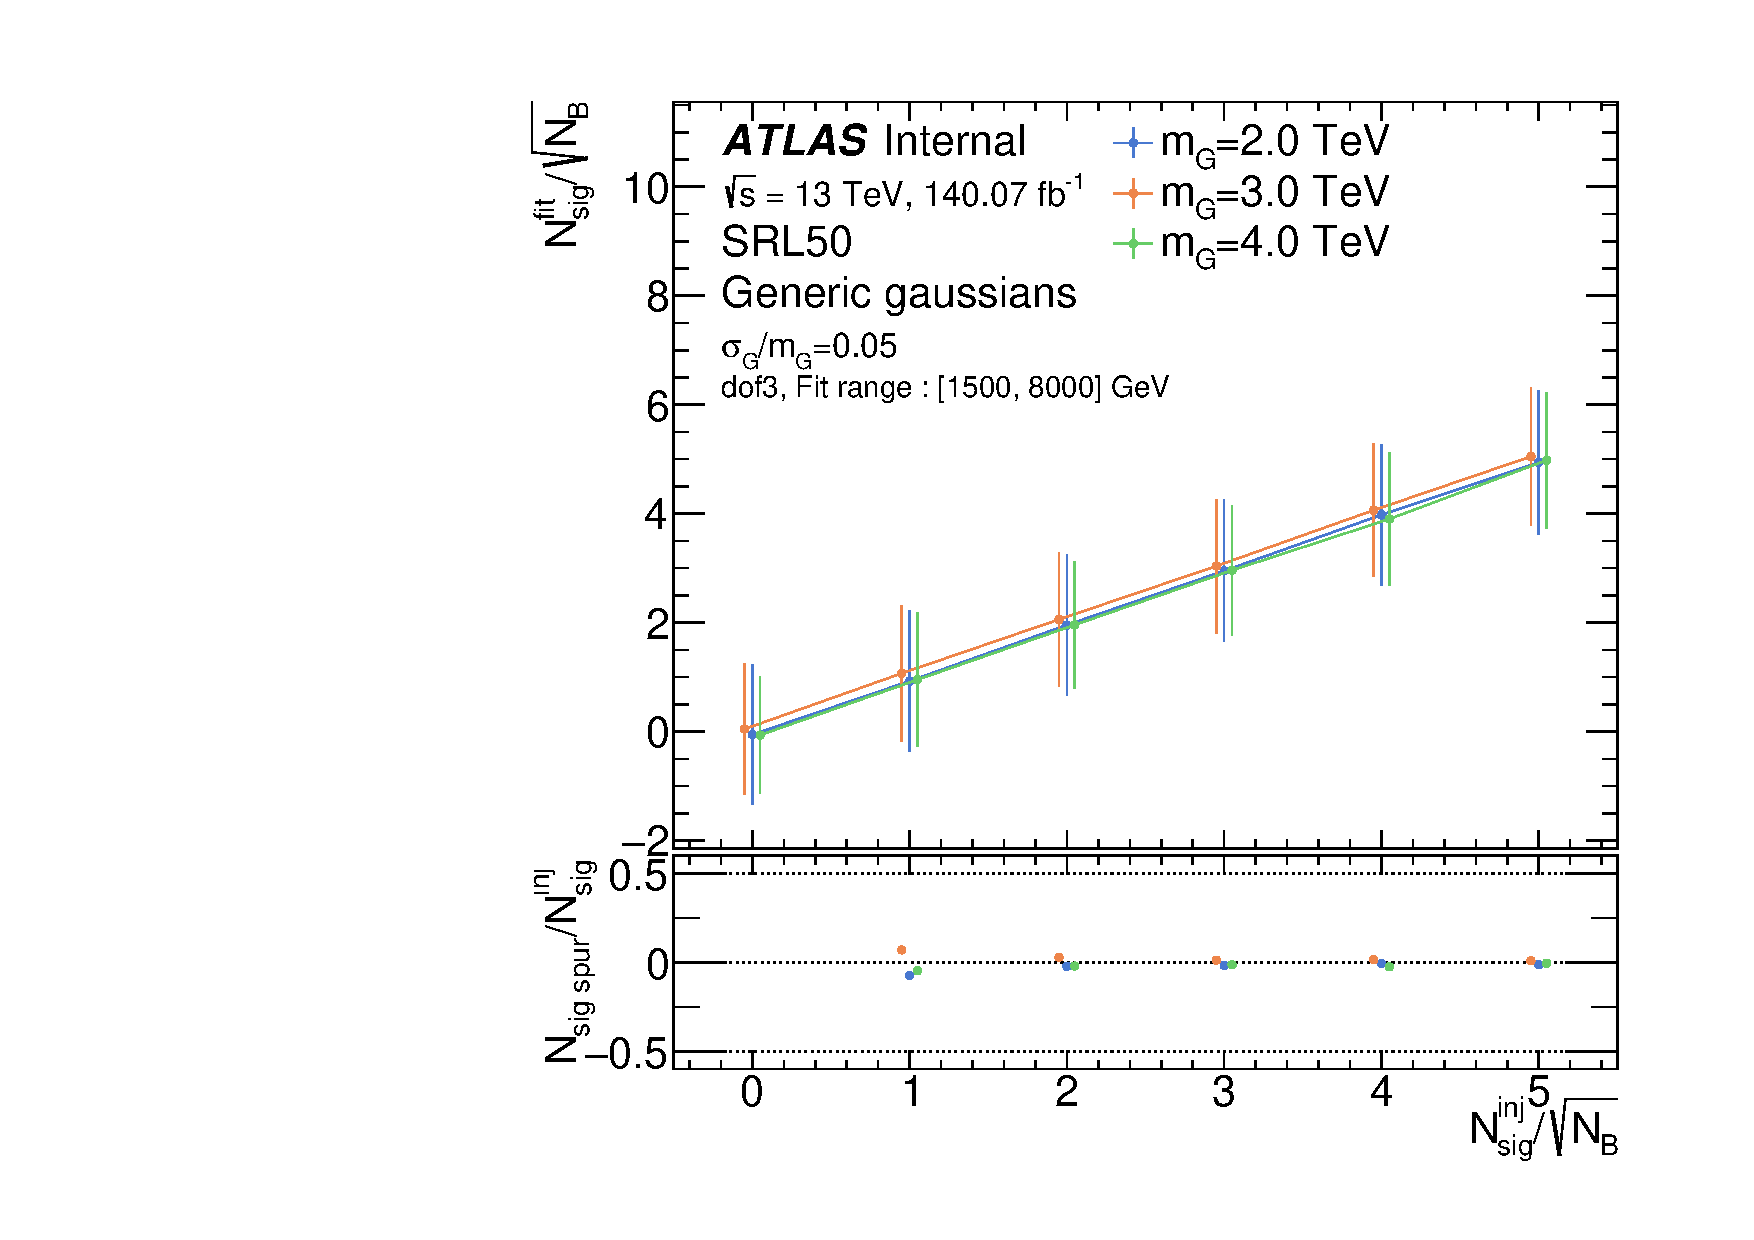
\includegraphics[width=\textwidth]{5_resonances/bkg/modeling/si/toys/SRL50/gaus/width0p05/dof3__range_1500_8000/plots/can__SigInj__photonjet_Pythia_jfakeisosmooth__gaus__SRL50__width0p05__dof3__range_1500_8000}
        \caption{\(\sigma_G/\mG = 0.05\).}
    \end{subfigure}
    \hfill
    \begin{subfigure}[h]{0.32\linewidth}
        \centering
        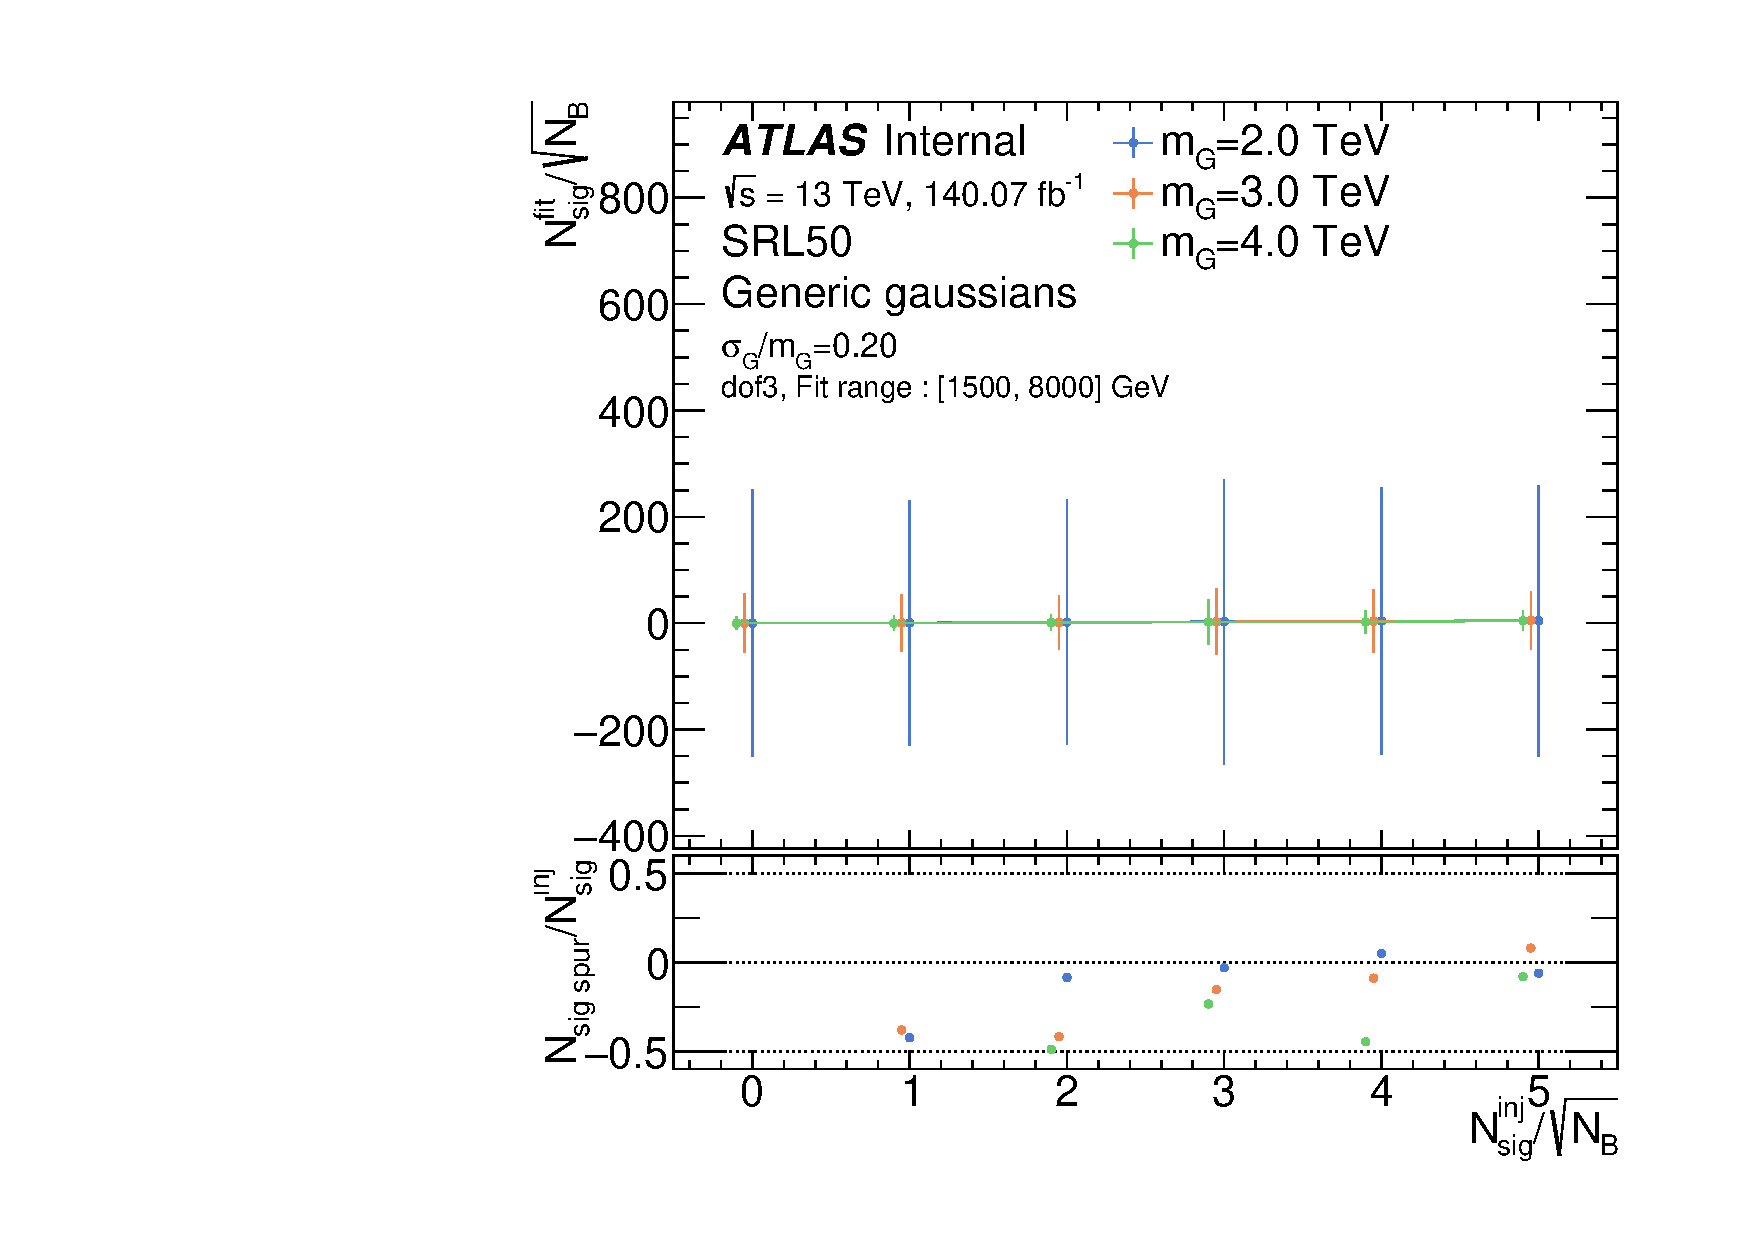
\includegraphics[width=\textwidth]{5_resonances/bkg/modeling/si/toys/SRL50/gaus/width0p20/dof3__range_1500_8000/plots/can__SigInj__photonjet_Pythia_jfakeisosmooth__gaus__SRL50__width0p20__dof3__range_1500_8000}
        \caption{\(\sigma_G/\mG = 0.20\).}
    \end{subfigure}
    \caption{\'Idem a la \Fig{\ref{fig:si_results:siginj_gaus_SR}} en la regi\'on SRL, realizando los ajustes en el rango de \(1500-8000~\gev\) y utilizando la funci\'on \textit{dof3}.}
    \label{fig:si_results:siginj_gaus_SRL}
\end{figure}

\begin{figure}[ht!]
    \centering
    \begin{subfigure}[h]{0.32\linewidth}
        \centering
        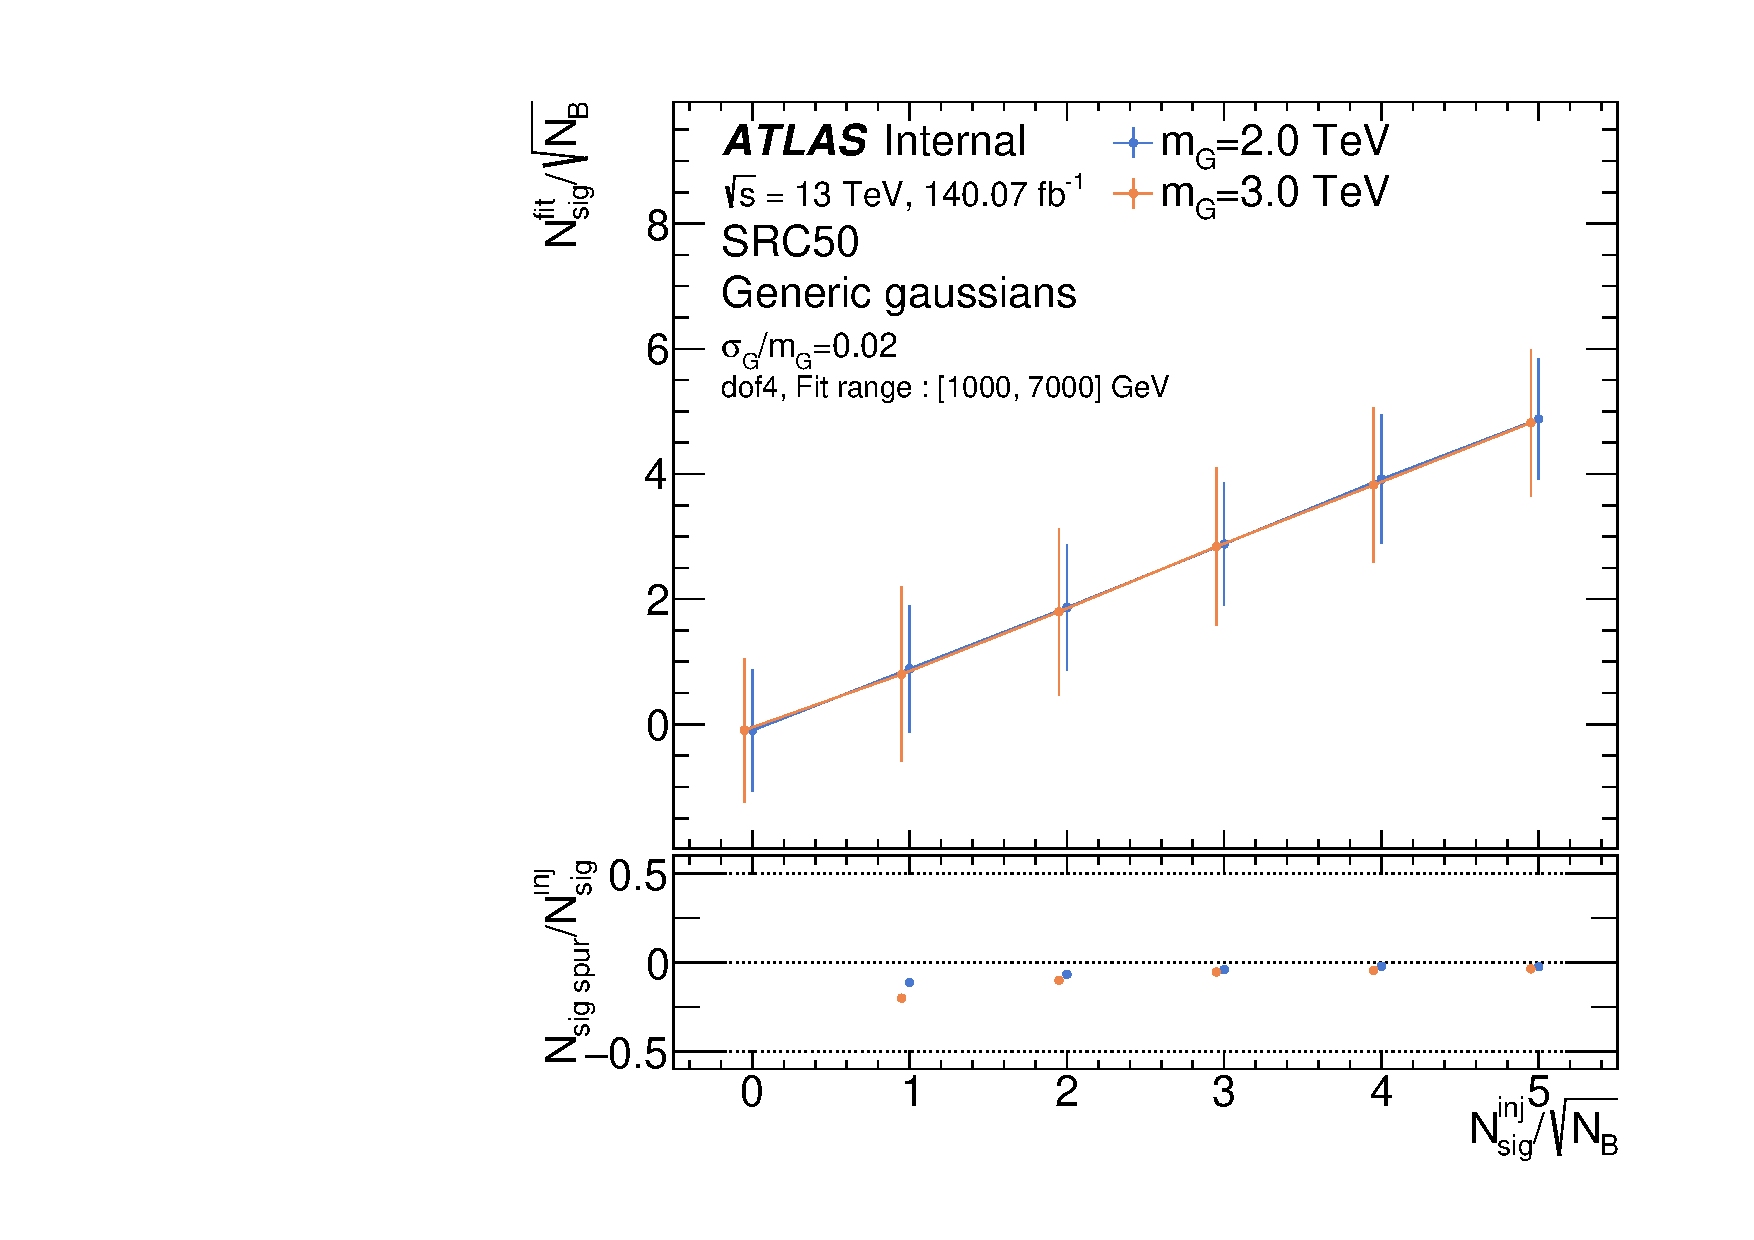
\includegraphics[width=\textwidth]{5_resonances/bkg/modeling/si/toys/SRC50/gaus/width0p02/dof4__range_1000_7000/plots/can__SigInj__photonjet_Pythia_jfakeisosmooth__gaus__SRC50__width0p02__dof4__range_1000_7000}
        \caption{\(\sigma_G/\mG = 0.02\).}
    \end{subfigure}
    \hfill
    \begin{subfigure}[h]{0.32\linewidth}
        \centering
        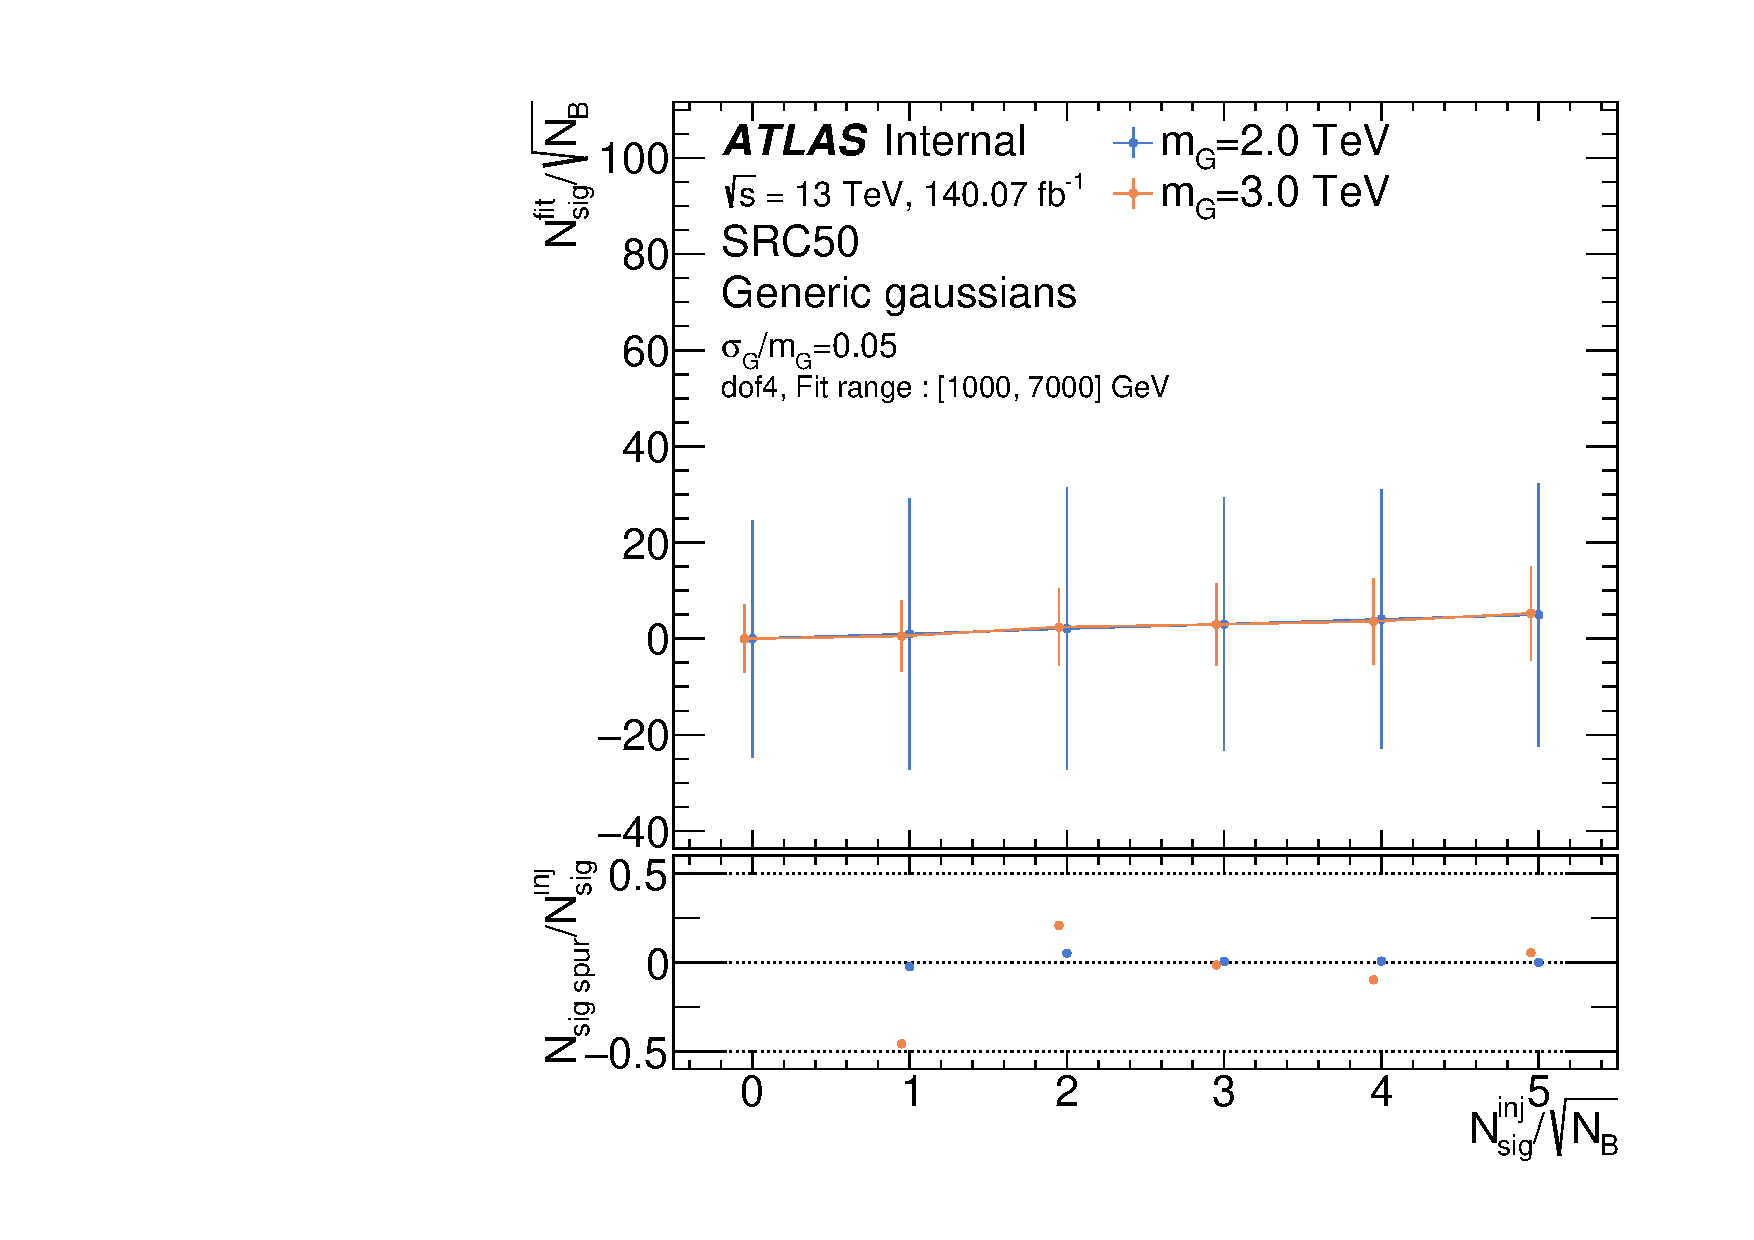
\includegraphics[width=\textwidth]{5_resonances/bkg/modeling/si/toys/SRC50/gaus/width0p05/dof4__range_1000_7000/plots/can__SigInj__photonjet_Pythia_jfakeisosmooth__gaus__SRC50__width0p05__dof4__range_1000_7000}
        \caption{\(\sigma_G/\mG = 0.05\).}
    \end{subfigure}
    \hfill
    \begin{subfigure}[h]{0.32\linewidth}
        \centering
        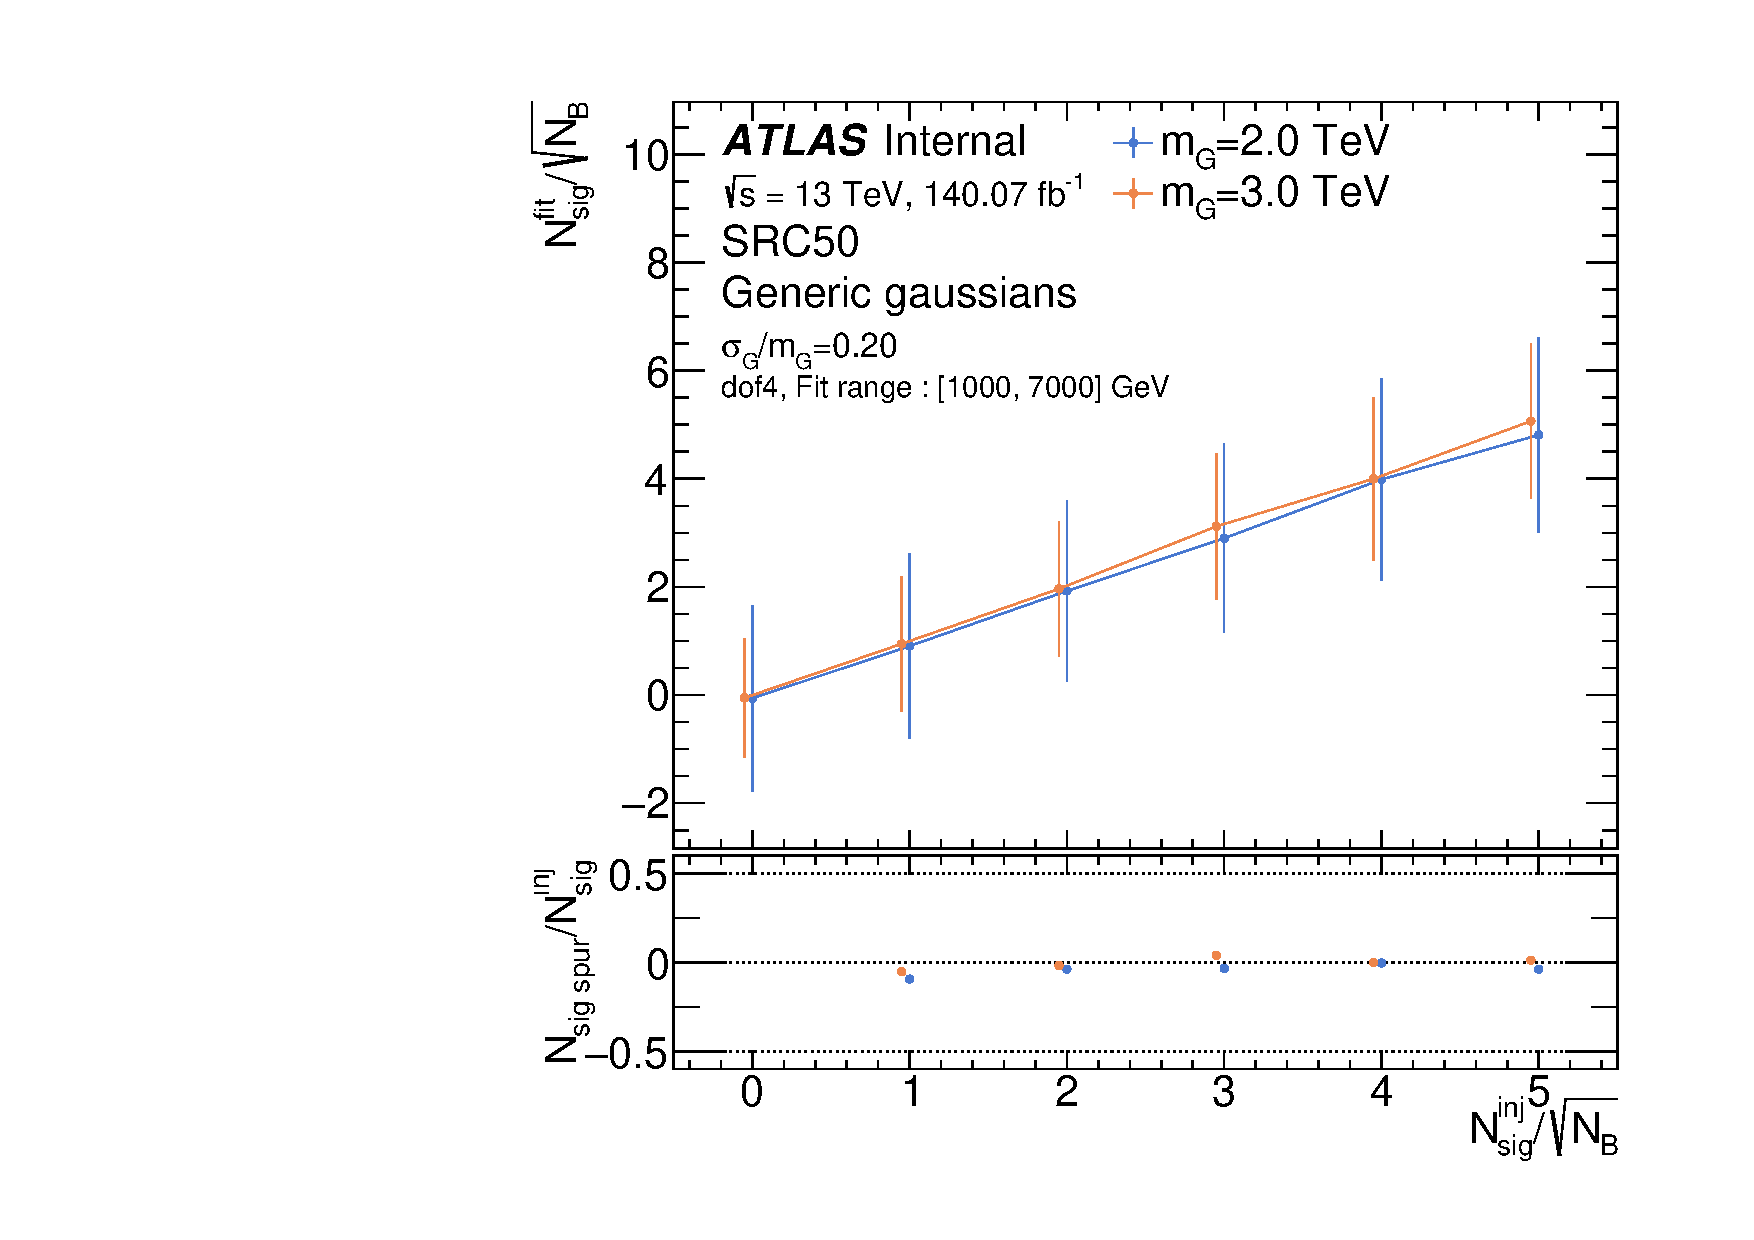
\includegraphics[width=\textwidth]{5_resonances/bkg/modeling/si/toys/SRC50/gaus/width0p20/dof4__range_1000_7000/plots/can__SigInj__photonjet_Pythia_jfakeisosmooth__gaus__SRC50__width0p20__dof4__range_1000_7000}
        \caption{\(\sigma_G/\mG = 0.20\).}
    \end{subfigure}
    \caption{\'Idem a la \Fig{\ref{fig:si_results:siginj_gaus_SR}} en la regi\'on SRC, realizando los ajustes en el rango de \(1000-7000~\gev\) y utilizando la funci\'on \textit{dof4}.}
    \label{fig:si_results:siginj_gaus_SRC}
\end{figure}

\begin{figure}[ht!]
    \centering
    \begin{subfigure}[h]{0.32\linewidth}
        \centering
        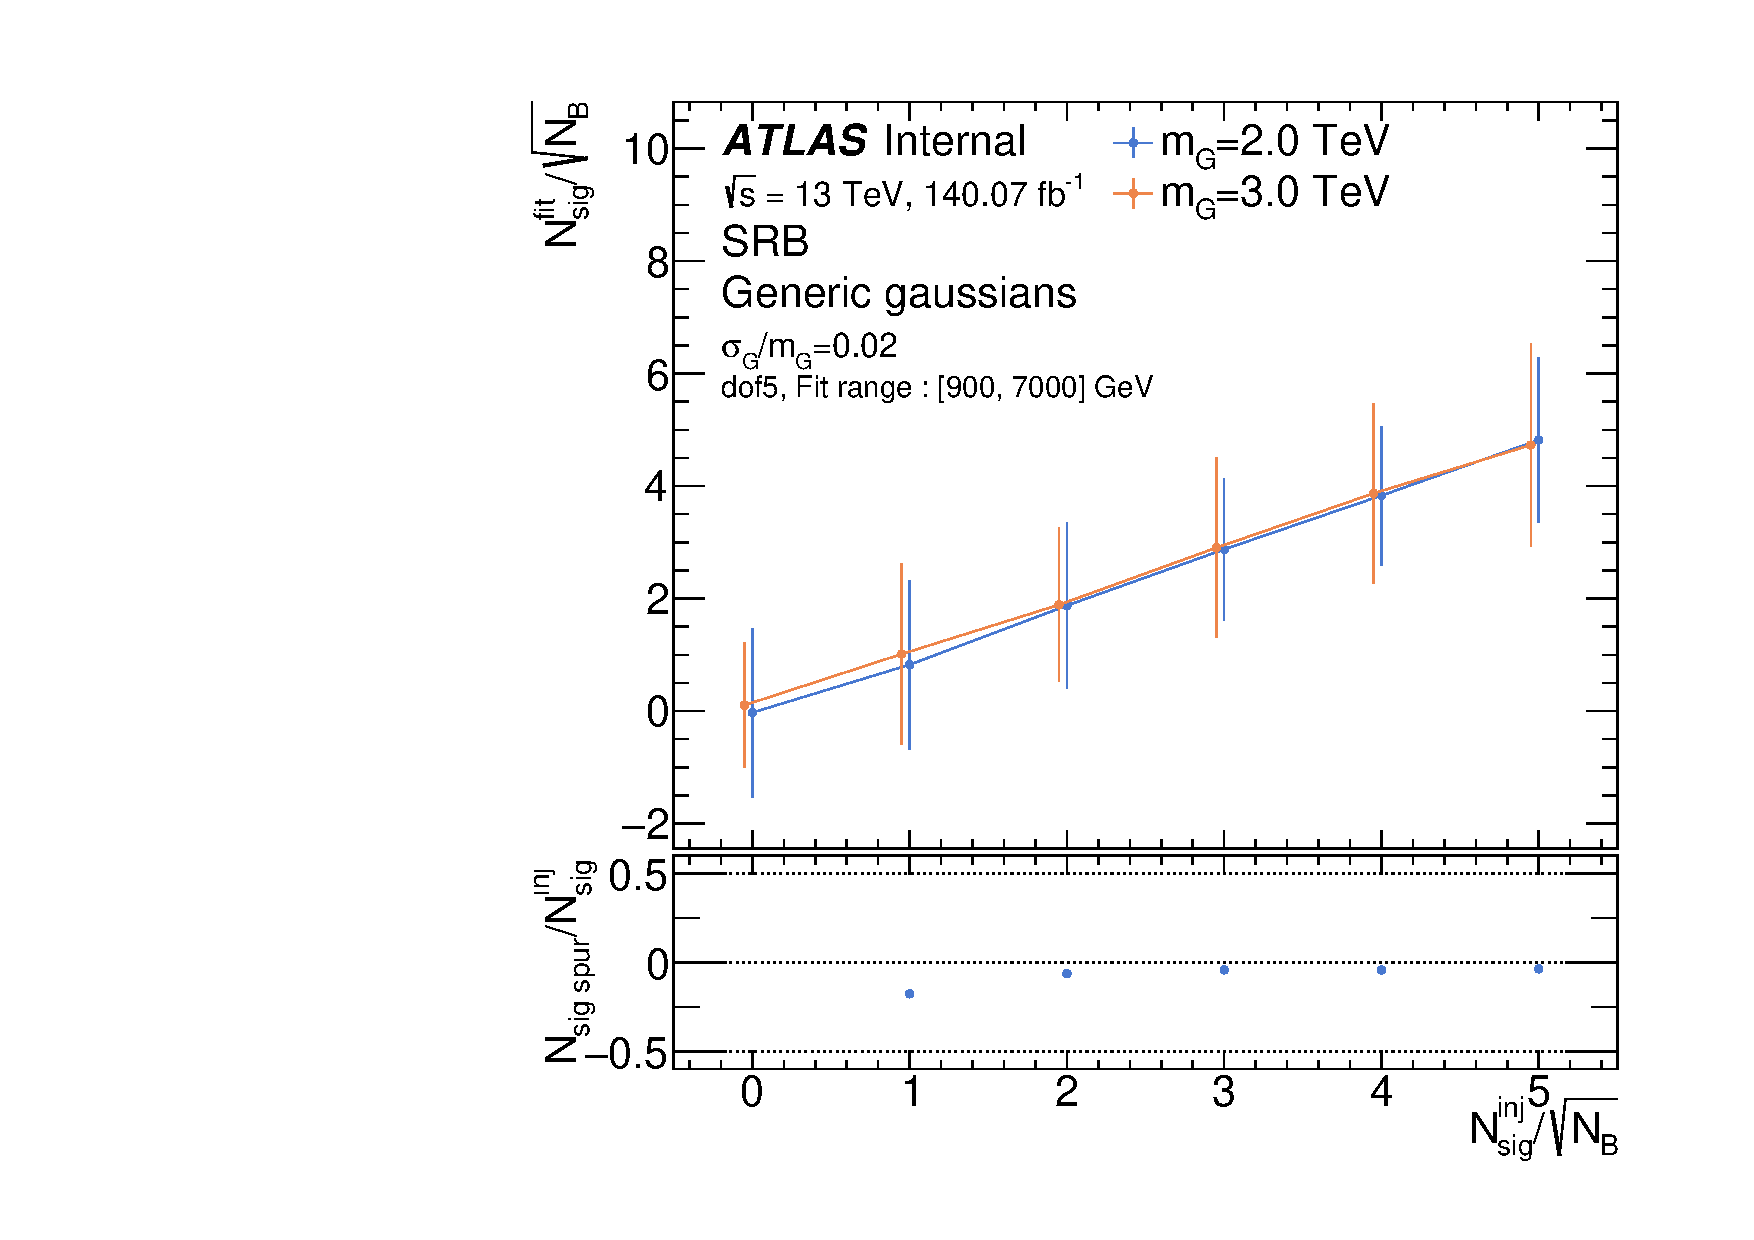
\includegraphics[width=\textwidth]{5_resonances/bkg/modeling/si/toys/SRB/gaus/width0p02/dof5__range_900_7000/plots/can__SigInj__photonjet_Pythia_jfakeisosmooth__gaus__SRB__width0p02__dof5__range_900_7000}
        \caption{\(\sigma_G/\mG = 0.02\).}
    \end{subfigure}
    \hfill
    \begin{subfigure}[h]{0.32\linewidth}
        \centering
        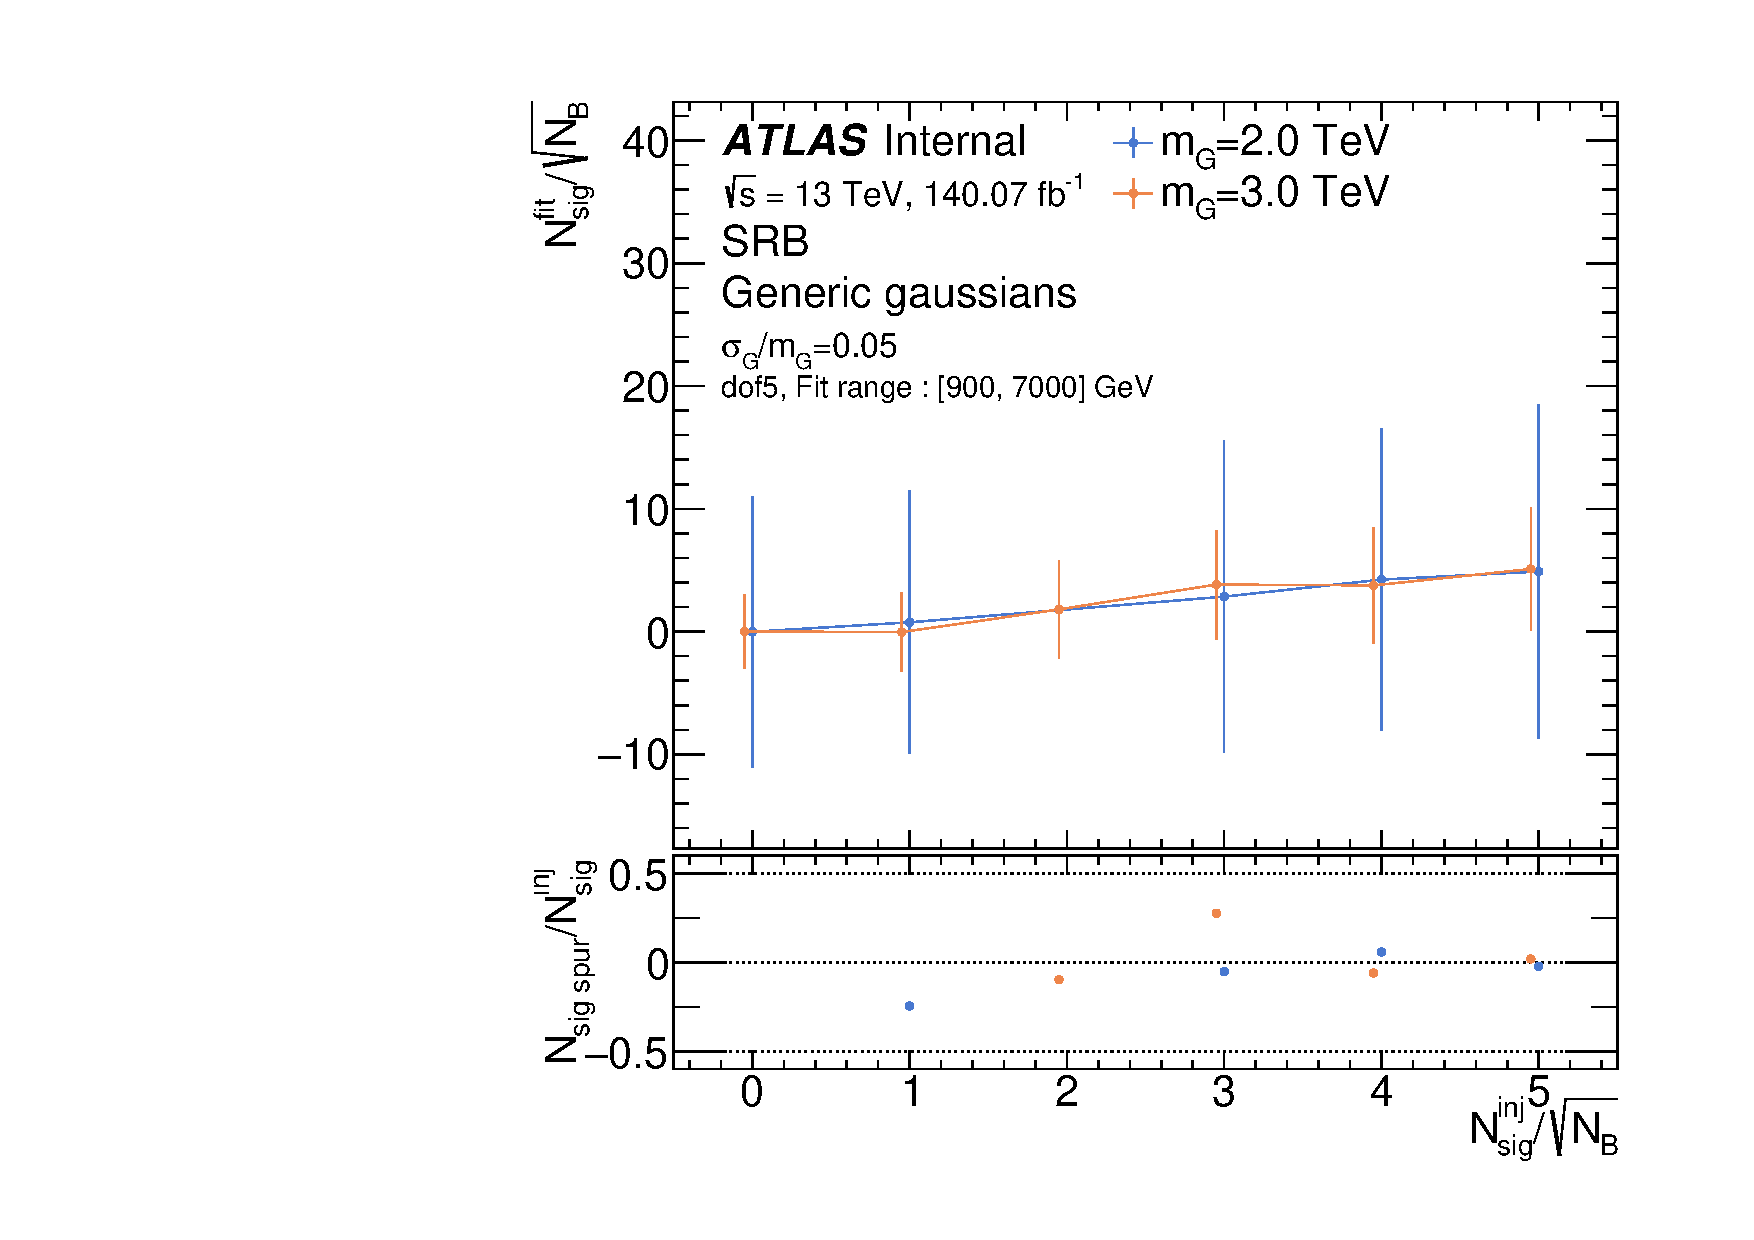
\includegraphics[width=\textwidth]{5_resonances/bkg/modeling/si/toys/SRB/gaus/width0p05/dof5__range_900_7000/plots/can__SigInj__photonjet_Pythia_jfakeisosmooth__gaus__SRB__width0p05__dof5__range_900_7000}
        \caption{\(\sigma_G/\mG = 0.05\).}
    \end{subfigure}
    \hfill
    \begin{subfigure}[h]{0.32\linewidth}
        \centering
        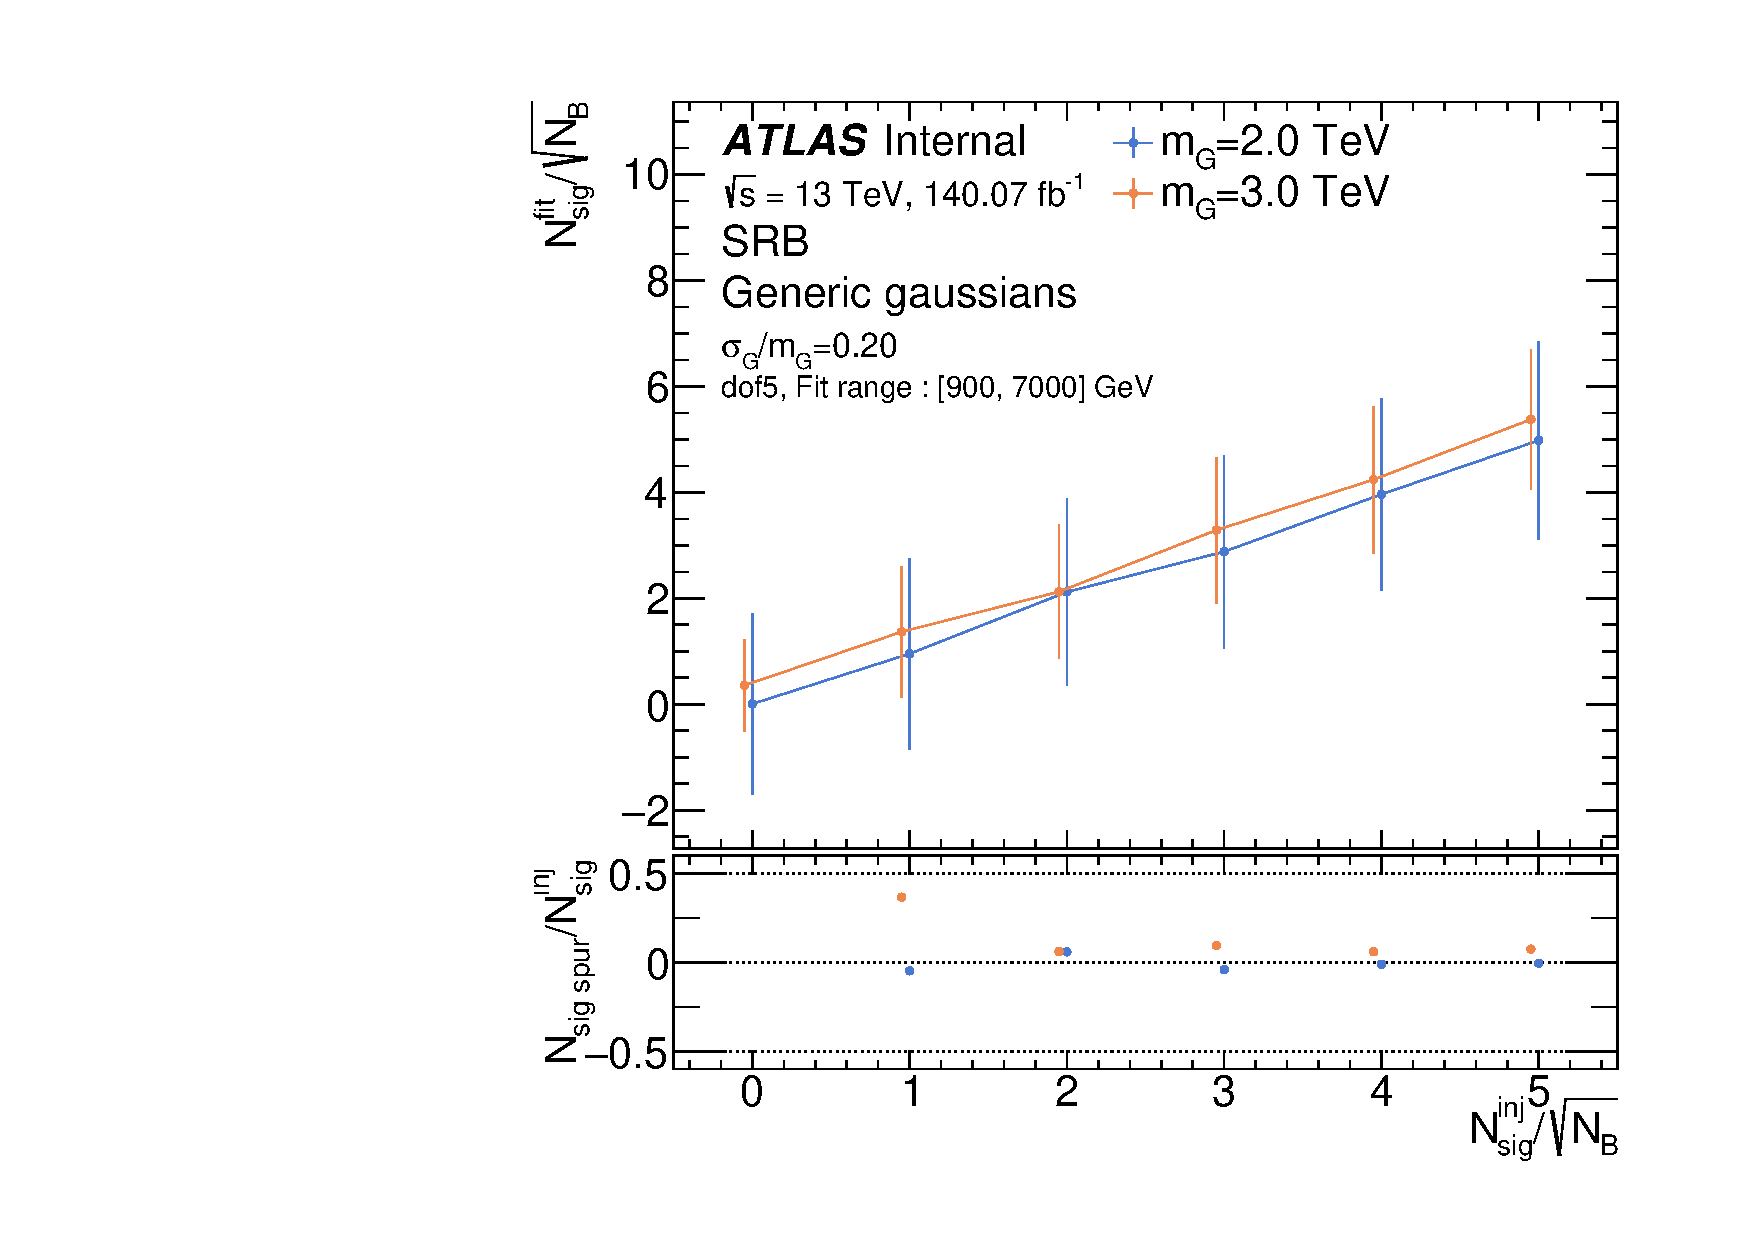
\includegraphics[width=\textwidth]{5_resonances/bkg/modeling/si/toys/SRB/gaus/width0p20/dof5__range_900_7000/plots/can__SigInj__photonjet_Pythia_jfakeisosmooth__gaus__SRB__width0p20__dof5__range_900_7000}
        \caption{\(\sigma_G/\mG = 0.20\).}
    \end{subfigure}
    \caption{\'Idem a la \Fig{\ref{fig:si_results:siginj_gaus_SR}} en la regi\'on SRB, realizando los ajustes en el rango de \(900-7000~\gev\) y utilizando la funci\'on \textit{dof5}.}
    \label{fig:si_results:siginj_gaus_SRB}
\end{figure}



\paragraph{Micro-Agujeros Negros}
De forma similar a lo que se ha visto para las señales gaussianas, en el caso \ac{QBH} se sigue una buena linealidad con todas las masas consideradas dentro del rango de ajuste.

\begin{figure}[ht!]
    \centering
    \begin{subfigure}[h]{0.49\linewidth}
        \centering
        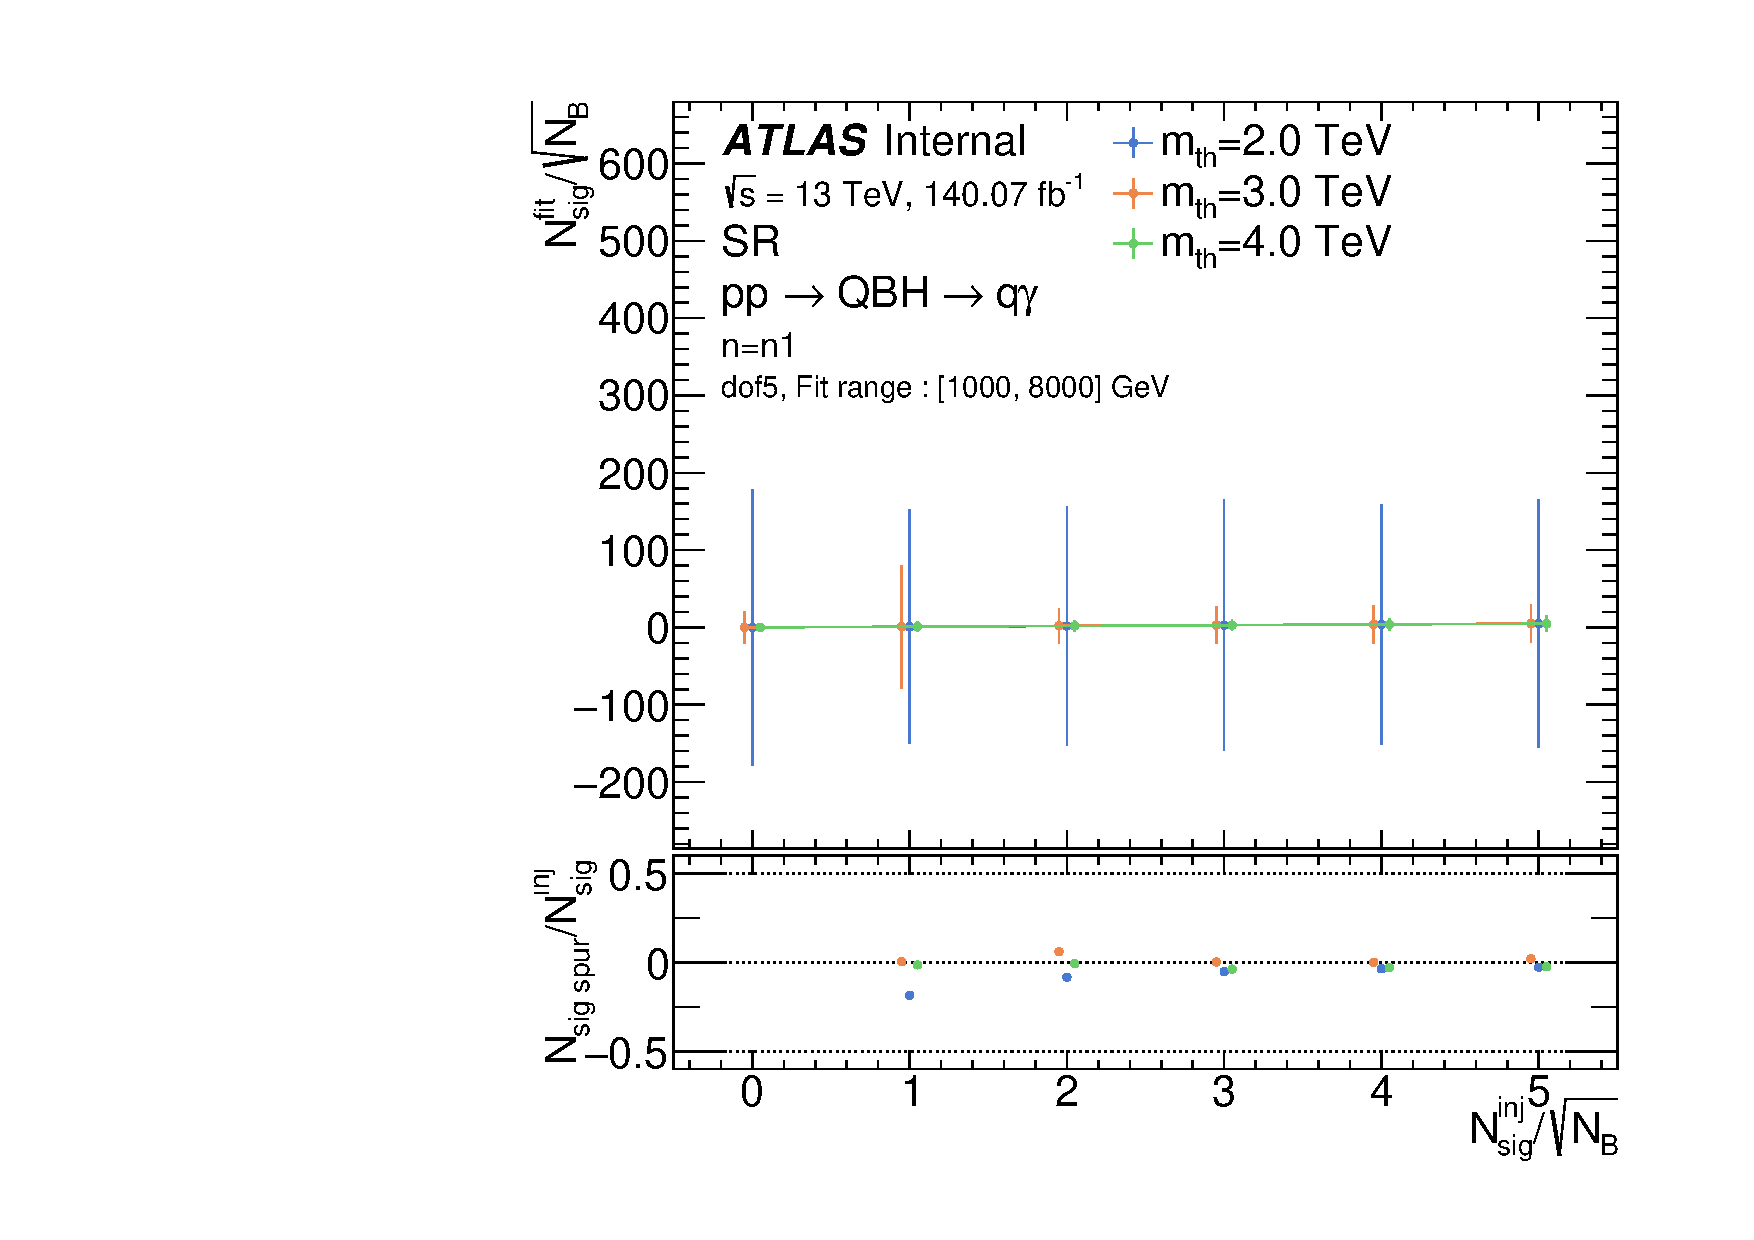
\includegraphics[width=\textwidth]{5_resonances/bkg/modeling/si/toys/SR/QBH/n1/dof5__range_1000_8000/plots/can__SigInj__photonjet_Pythia_jfakeisosmooth__QBH__SR__n1__dof5__range_1000_8000}
        \caption{\(n = 1\) (RS1).}
    \end{subfigure}
    \hfill
    \begin{subfigure}[h]{0.49\linewidth}
        \centering
        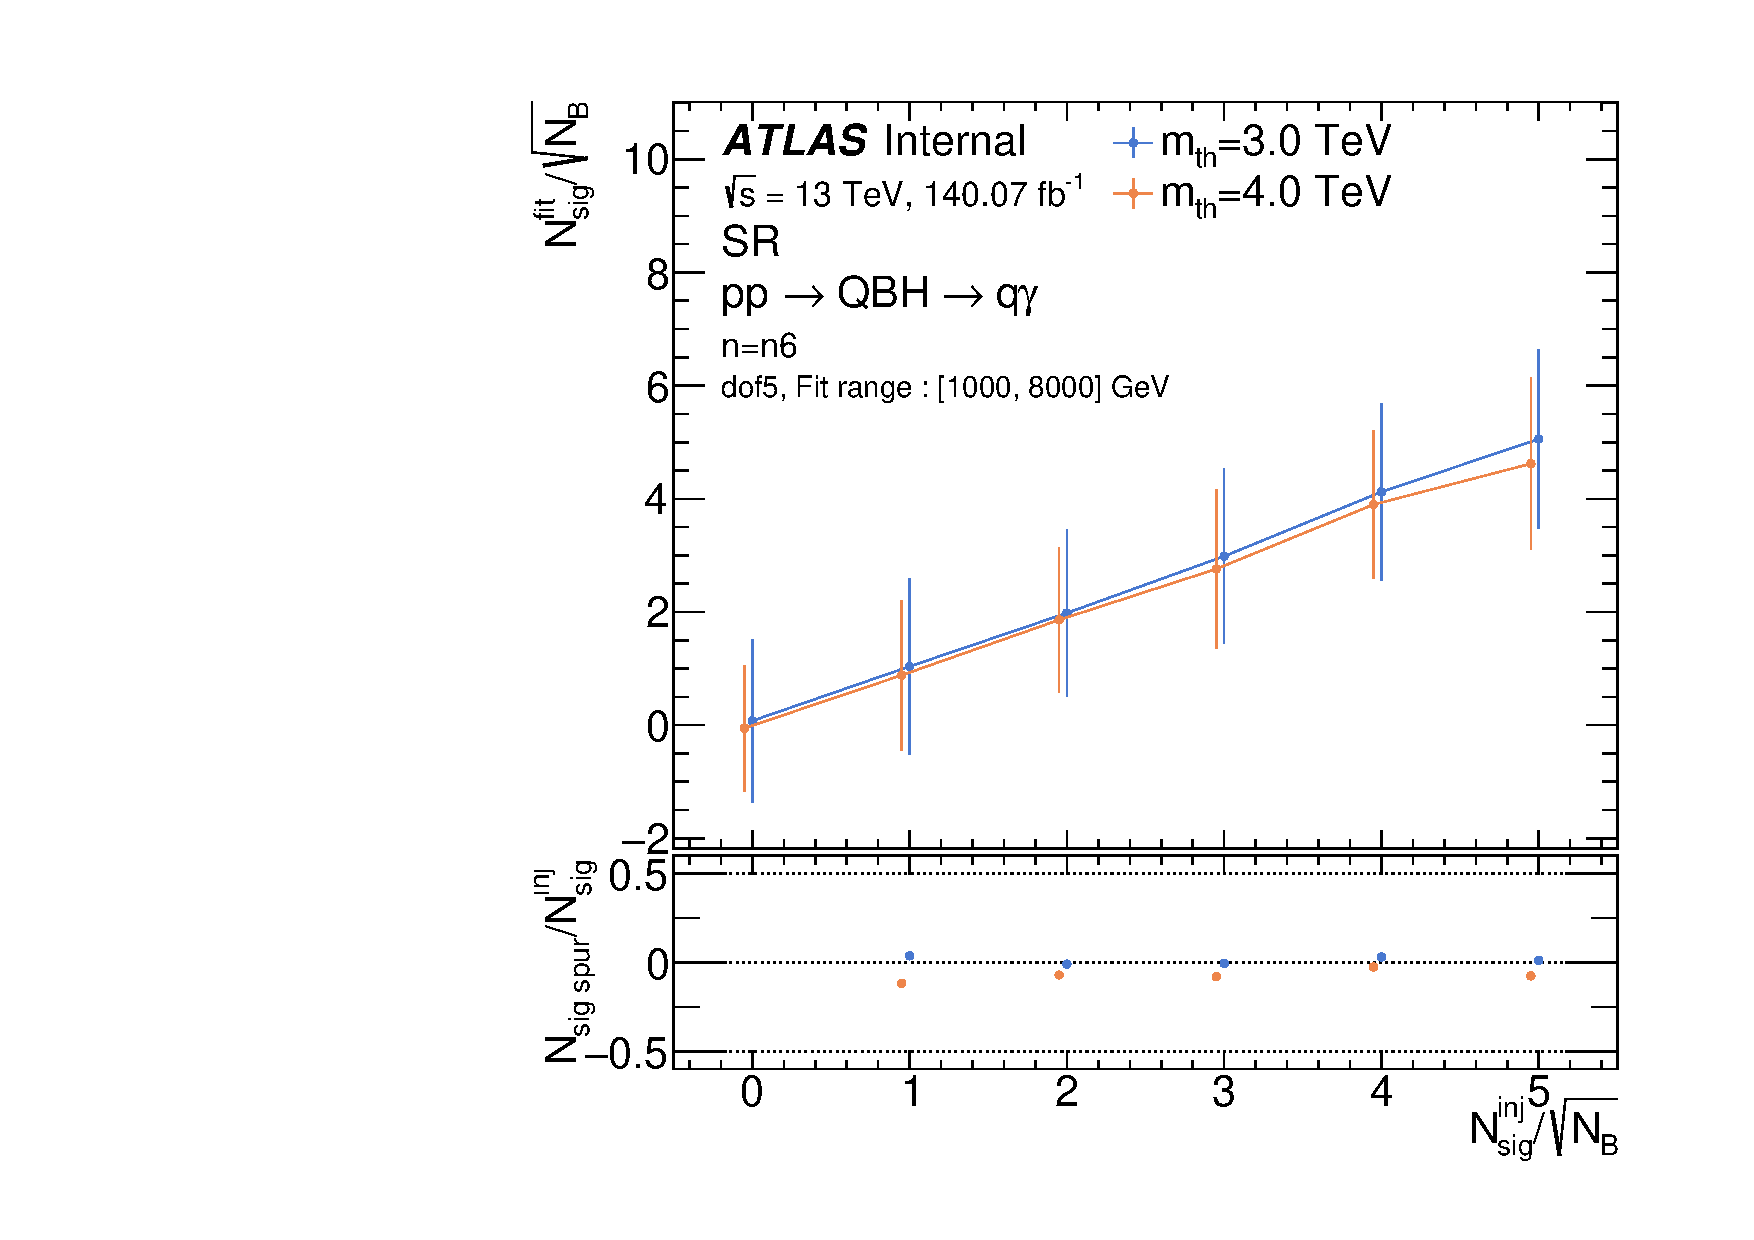
\includegraphics[width=\textwidth]{5_resonances/bkg/modeling/si/toys/SR/QBH/n6/dof5__range_1000_8000/plots/can__SigInj__photonjet_Pythia_jfakeisosmooth__QBH__SR__n6__dof5__range_1000_8000}
        \caption{\(n = 6\) (ADD).}
    \end{subfigure}
    \caption{Resultados del test de \ac{SI} utilizando las se\~nales de \ac{QBH} en la regi\'on inclusiva SR. El ajuste se realiza en el rango \(1000-8000~\gev\) utilizando la funci\'on \textit{dof5}.}
    \label{fig:si_results:siginj_QBH_SR}
\end{figure}